\documentclass[12pt,a4paper]{ctexart}

% 基础宏包
\usepackage{geometry}
\geometry{left=2.5cm,right=2.5cm,top=2.5cm,bottom=2.5cm}

% 数学宏包
\usepackage{amsmath,amssymb,amsfonts,amsthm}

% 图表宏包
\usepackage{graphicx}
\usepackage{booktabs}
\usepackage{longtable}
\usepackage{multirow}
\usepackage{array}
\usepackage{float}

% 颜色与样式
\usepackage{xcolor}
\usepackage{tikz}
\usetikzlibrary{shapes.geometric, arrows.meta, positioning, calc, fit, backgrounds}

% 超链接（黑色无边框，保留可点击跳转功能）
\usepackage[hidelinks]{hyperref}

% 参考文献（使用 natbib + 自定义上角标命令模拟 GB/T 7714-2015）
\usepackage[numbers,sort&compress]{natbib}
\bibliographystyle{unsrtnat}

% 上角标引用命令（GB/T 7714-2015 顺序编码制样式）
\newcommand{\upcite}[1]{\textsuperscript{\citep{#1}}}

% 将 \cite 重定义为 \upcite
\let\cite\upcite

% 代码与算法
\usepackage{listings}
% \usepackage{algorithm}
% \usepackage{algpseudocode}

% 标题格式
\usepackage{titlesec}

% 页眉页脚
\usepackage{fancyhdr}
\pagestyle{fancy}
\fancyhf{}
\fancyhead[C]{\small 宏观经济变量与沪深300指数收益率研究}
\fancyfoot[C]{\thepage}

% 交叉引用增强
\usepackage{cleveref}

% 图表标题
\usepackage{caption}
\captionsetup{font=small,labelfont=bf}

% 三线表专用
\newcommand{\topline}{\toprule[1.2pt]}
\newcommand{\midline}{\midrule[0.8pt]}
\newcommand{\bottomline}{\bottomrule[1.2pt]}

% 定理环境
\newtheorem{theorem}{定理}
\newtheorem{lemma}{引理}
\newtheorem{proposition}{命题}
\newtheorem{definition}{定义}

% 文档信息
\title{\textbf{宏观经济变量与沪深300指数收益率：\\基于MIDAS模型的两阶段实证分析}}
\author{}
\date{}

\begin{document}

\maketitle

\begin{abstract}
\noindent 股票市场收益率与宏观经济变量之间的关系始终是金融研究中的重要议题。围绕这一问题，本文以沪深300指数为研究对象，构建"宏观变量形成收益预期---市场状态解释预期偏离"的两阶段实证分析框架，尝试从基本面信息与市场实现之间的动态关系出发，考察短线与长线收益窗口下宏观信息、资金行为、情绪波动和流动性状态的不同作用路径。研究样本覆盖2015年7月至2025年12月的日度交易数据，结合月度宏观指标、市场情绪指标、隐含波动率、北向资金、融资融券余额及流动性变量，形成可用于混频建模与偏离解释的统一分析样本。

在研究方法上，第一阶段采用MIDAS混频回归模型，将CPI、PPI、M2同比增速、经济政策不确定性指数以及美元兑人民币汇率等月度宏观变量引入未来5日和60日累计收益率预测方程，通过参数化权重函数刻画低频宏观信息在不同滞后期上的影响强度，并在样本内与样本外两个维度比较单变量模型和精简多变量模型的预测表现。第二阶段以第一阶段生成的条件预期收益率为基准，重新构造异常收益及异常收益绝对值，进一步采用分组嵌套回归识别情绪与风险感知、资金与杠杆交易、流动性与交易状态等变量对收益偏离的边际解释作用，同时结合Newey--West HAC稳健标准误处理重叠收益窗口所带来的序列相关问题。

从研究设计与数据分析结果看，宏观变量进入高频收益率预测时具有明显的期限差异：短窗口收益更易受到交易层面扰动，较长窗口对宏观信息的吸收更充分。市场状态变量之间存在一定相关性，分组嵌套框架更便于识别不同机制的边际贡献。后续实证将在这一基础上进一步比较不同宏观变量在5日与60日窗口中的预测表现，并检验情绪、隐含波动率、资金流向和非流动性因素对异常收益偏离强度的解释能力。

\vspace{1em}
\noindent\textbf{关键词：}MIDAS模型；沪深300指数；收益率预测；宏观经济变量；异常收益偏离；投资者情绪
\end{abstract}

\thispagestyle{fancy}

\newpage
\tableofcontents
\newpage

% 引入各章节
% 第一章 绪论、文献综述与研究方法

\section{绪论、文献综述与研究方法}

\subsection{引言}

股票市场收益率与宏观经济变量之间的关系，始终是金融研究中的重要议题。经典研究已经表明，股票预期收益并非固定不变，而会随着商业周期、风险溢价与整体经济状态的变化而调整。\cite{fama1989business}发现，股票与长期债券的预期收益呈现出清晰的商业周期特征，经济环境偏弱时预期收益较高，经济状况偏强时预期收益相对较低，这说明宏观状态能够系统性地进入资产定价过程。随后，大量研究继续围绕收益预测问题展开讨论。\cite{campbell2008predicting}认为，在预测回归中加入适度的经济约束后，部分变量仍能在样本外提供有限但具有经济意义的预测增益；\cite{welch2008comprehensive}则指出，许多变量虽然在样本内表现突出，却难以持续稳定地优于历史均值模型。这些研究共同提示，宏观变量更适合作为收益率条件预期的构造基础。

这一问题在中国资本市场中具有更强的现实意义。A股市场长期表现出较高的政策敏感性、情绪波动性和资金驱动特征，宏观变量、政策预期、汇率变化以及市场风险情绪之间往往存在更为紧密的互动。随着北向资金持续进入、期权市场逐步扩容以及高频交易信息不断丰富，市场价格形成机制已经同时包含宏观基本面、跨境资金流、投资者情绪和流动性摩擦等多重因素。近年的中国研究也表明，宏观经济不确定性在A股市场中存在显著定价效应，北向资金会改变市场流动性和价格表现，投资者情绪及信息环境也会进一步影响收益形成机制\cite{ge2024macroeconomic,yang2023northbound,he2024timevarying}。在这一背景下，研究宏观信息如何形成收益预期、市场为何偏离这一预期，具有明显的理论价值和现实意义。

基于上述认识，本文将研究重点放在两个相互衔接的环节。第一阶段利用月度宏观经济变量构建沪深300指数未来5日与60日累计收益率的条件预期；第二阶段以实际收益率与条件预期收益率之差构造异常收益及其绝对值，并进一步检验市场情绪、风险感知、资金流向、杠杆交易、流动性和交易状态等因素对收益偏离的解释作用。这样的处理能够将"基本面信息进入收益率"的过程与"市场围绕基本面发生偏离"的过程区分开来，也有助于更清楚地刻画短线与长线收益波动的形成机制。

\subsection{研究现状与文献综述}

\subsubsection{宏观经济变量与股票收益率预测研究}

宏观经济变量能否预测股票收益率，是资产定价与经验金融研究中的经典问题。\cite{fama1989business}较早将股票收益与商业周期联系起来，指出预期收益具有明显的宏观状态依赖性。在此基础上，\cite{campbell2008predicting}从样本外预测角度重新讨论了收益预测问题，认为若在模型中施加合理的经济约束，部分预测回归在样本外仍可取得一定改进。\cite{welch2008comprehensive}则系统比较了权益溢价预测变量的经验表现，发现许多变量在样本内看似有效，但在样本外往往难以持续优于历史均值。由此形成的基本共识是，宏观变量对股票收益率的作用更多体现为条件预期的变化，而非一种简单、固定、线性的决定关系。

国内研究同样表明，宏观变量在中国股票市场中具有重要作用，但这种作用往往带有更强的状态依赖性和阶段差异。\cite{ge2024macroeconomic}基于中国A股市场数据构建宏观经济不确定性指标后发现，宏观不确定性暴露存在显著溢价效应，而且这一效应会随公司特征和市场环境变化而发生异质性调整。这些研究说明，在中国市场中讨论宏观变量与股票收益率的关系时，单一平均效应往往不足以捕捉真实机制，将宏观信息置于"条件预期收益率"的框架中进行处理，更符合当前经验研究的发展方向。

\subsubsection{混频数据模型与 MIDAS 方法研究}

宏观变量预测金融市场收益率时面临的直接难题，在于数据频率不一致。宏观指标通常以月度或季度发布，而股票收益率则以日度持续变动。如果直接将低频变量机械复制到高频样本中，既无法充分体现宏观信息的动态传导，也会扭曲信息到达顺序。\cite{ghysels2004midas,ghysels2006midas}提出的 MIDAS 模型，为不同频率数据的联合建模提供了系统方法。该模型通过参数化权重函数，将低频变量的多个滞后期压缩到高频回归方程中，从而在保留时序结构信息的同时避免参数维数过快膨胀。随后，\cite{ghysels2007midas}对 MIDAS 回归的估计和应用进行了进一步拓展，说明其不仅适用于波动率预测，同样适用于一般意义上的收益率和宏观变量预测。\cite{schorfheide2015realtime}则从实时预测角度比较了 mixed-frequency VAR 与 MIDAS 回归，指出混频框架在处理宏观信息逐步披露时具有明显优势。

在中国语境下，混频方法也已经获得较为稳固的应用基础。\cite{zheng2013midas}将 MIDAS 模型用于中国 GDP 的短期预测，发现基于金融变量的 MIDAS 模型在实时数据背景下具有较好的预测表现，并且多元扩展模型在若干设定下优于基准模型。这一结果说明，MIDAS 方法在中国宏观金融数据环境中具有较好的可操作性。本文主要从两个方面使用这一方法：其一，月度宏观变量能够与日度收益窗口直接对接；其二，过去若干期宏观信息的影响强度可以通过权重函数灵活刻画，从而更贴合宏观冲击对市场收益率并非一次性释放的现实特征。

\subsubsection{投资者情绪、风险感知与收益偏离研究}

在经典资产定价框架之外，行为金融研究强调，投资者情绪会改变资产定价并推动价格偏离基本面。\cite{baker2006investor}的研究表明，情绪波动对那些估值主观性强、套利难度较高的资产影响更为显著，这意味着市场价格围绕基本面发生偏离，也与投资者风险偏好和情绪波动直接相关。

这一研究路径在中国市场得到了进一步扩展。\cite{wang2004investor}较早指出，投资者情绪会显著影响我国股市收益与收益波动。\cite{yin2019highfrequency}利用高频情绪指标发现，投资者高频情绪对股票日内收益率具有明显预测作用。\cite{mei2019investor}基于移动互联网文本构造情绪指标，发现乐观情绪越高，下一期股票收益越高，而且这种作用在信息环境较差、流动性较弱的股票上更为突出。相关研究表明，在中国股票市场中，情绪和风险感知会直接影响收益率的实现路径。对于本文的研究设计而言，情绪变量更适合放在第二阶段，用于解释市场为何围绕宏观条件预期发生偏离。

\subsubsection{资金流向、流动性与交易状态研究}

除情绪因素外，资金流向和市场流动性同样会显著影响收益率表现。\cite{amihud2002illiquidity}从时间序列和横截面两个层面说明，预期市场非流动性上升会提高投资者要求的回报补偿，股票收益中包含明确的流动性溢价。这一结果在后续研究中得到多次验证，也使流动性成为理解收益偏离和市场异动的重要视角。

在中国市场中，北向资金的作用受到越来越多关注。\cite{yang2023northbound}基于高频数据研究发现，北向资金整体上能够提升股票流动性，其作用机制主要体现在信息机制和竞争机制，但在特定情境下也可能通过价格冲击和筹码约束影响市场质量。\cite{he2024timevarying}进一步指出，北向资金与中国股市表现之间存在时变互动关系，其对收益的影响具有明显短期性，并在极端波动时期呈现出一定的稳定市场特征。这些研究提示，资金流向、杠杆交易与流动性状态不仅影响收益率本身，也会影响市场围绕宏观基本面形成预期偏离的幅度和持续性。

\subsubsection{文献评述}

现有研究已经形成较为完整的理论与方法基础。宏观收益预测文献关注经济状态如何进入条件预期，MIDAS 研究解决了低频宏观变量与高频收益率之间的频率衔接问题，情绪、资金与流动性研究则揭示了市场围绕基本面发生偏离的多种机制。现有成果仍留下几处值得继续推进的空间。首先，许多研究聚焦月度或季度收益率，对未来5日与60日累计收益率这种"短线—长线并置"的预测窗口关注不足。其次，宏观收益预测研究与市场偏离解释研究往往分开展开，前者着重于预测能力，后者偏重于行为和微观结构因素，较少在同一框架中先构造宏观条件预期，再单独检验非基本面因素如何放大偏离。最后，针对中国股票市场的研究虽然已经涉及宏观不确定性、投资者情绪、北向资金和流动性等关键变量，但把这些因素纳入统一的两阶段实证框架中进行比较分析的研究仍相对有限。本文的研究路径正是在上述文献基础上的进一步延伸。

\subsection{研究方法与技术路线}

本文采用两阶段实证框架。第一阶段围绕"宏观变量如何形成收益预期"展开，第二阶段关注"市场为何偏离这一预期"。

在第一阶段，本文选取 CPI、PPI、M2增速、经济政策不确定性指数和美元兑人民币汇率等月度宏观变量作为核心信息集，利用 MIDAS 混频回归模型预测沪深300指数未来5日和60日累计收益率。考虑到宏观变量对未来收益率的影响可能具有不同的滞后分布，本文使用参数化权重函数对过去12个月的宏观信息进行加权，并分别构建单变量 MIDAS 模型。在此基础上，再根据样本内拟合效果、样本外递推表现、VIF 检验结果以及变量的经济含义，筛选出最多4个变量进入精简多变量模型，形成未来5日和60日累计收益率的条件预期值。样本外预测采用扩展窗口法，以前60\%的样本作为初始估计区间，对后40\%的样本进行动态递推，并使用 RMSE、MAE 和样本外 $R^2$ 等指标评价模型表现\cite{ghysels2004midas,zheng2013midas}。

在第二阶段，本文根据第一阶段生成的条件预期收益率构造异常收益和异常收益绝对值。未来 $h$ 日异常收益定义为
\begin{equation}
AR_t^{(h)}=R_t^{(h)}-\widehat{R}_t^{(h)},\qquad h\in\{5,60\}
\label{eq:abnormal_return}
\end{equation}
同时定义异常收益绝对值
\begin{equation}
AbsAR_t^{(h)}=\left|AR_t^{(h)}\right|
\label{eq:abs_abnormal_return}
\end{equation}
其中，$AR_t^{(h)}$ 反映偏离方向，$AbsAR_t^{(h)}$ 刻画偏离强度。考虑到偏离强度更能反映市场异动和风险放大过程，本文在主结果中以 $AbsAR_t^{(5)}$ 和 $AbsAR_t^{(60)}$ 作为核心因变量，在补充分析中再讨论带方向的异常收益。第二阶段解释变量按经济含义划分为三组：情绪与风险感知变量，包括情绪标准分和隐含波动率指数；资金与杠杆交易变量，包括北向资金净流入和融资融券余额；流动性与交易状态变量，包括 Amihud 非流动性指标、20日动量和日内振幅。回归设计采用分组嵌套方式，先检验情绪与风险感知变量，再逐步加入资金与杠杆交易变量、流动性与交易状态变量，并在完整嵌套模型之后通过 LASSO 辅助筛选非零系数变量。新增变量组的边际解释力通过增量联合检验与调整后 $R^2$ 的变化共同判断。由于未来5日和60日收益窗口都属于重叠窗口，第二阶段回归统一采用 Newey--West HAC 稳健标准误进行修正\cite{he2024timevarying,amihud2002illiquidity}。

整个研究的技术路线可以概括为五个环节。第一步，基于沪深300指数收盘价构造未来5日和60日累计收益率，并将月度宏观变量按照"上一个完整月可得信息"原则与日度样本对齐。第二步，将样本划分为训练集与测试集，在训练集上完成缩尾阈值计算、标准化参数估计、VIF 检验和单变量 MIDAS 估计，并将相应处理规则外推到测试集。第三步，利用单变量与精简多变量 MIDAS 模型形成宏观条件预期收益率。第四步，在此基础上构造异常收益及其绝对值，形成市场偏离指标。第五步，采用分组嵌套回归、增量联合检验、LASSO筛选和稳健性分析识别情绪、资金、流动性和交易状态对偏离的解释作用。这一技术路线将宏观信息、收益预期和市场异动纳入同一分析框架，研究目标与方法设定之间的对应关系也更清晰。

% 图1-1：研究技术路线图
\begin{figure}[htbp]
\centering
\begin{tikzpicture}[
    node distance=0.8cm and 1.2cm,
    box/.style={rectangle, rounded corners, draw=blue!60, fill=blue!5, very thick, minimum width=3cm, minimum height=0.8cm, align=center, font=\small},
    arrow/.style={-{Stealth[length=2mm]}, thick, blue!60}
]

% 第一行
\node[box] (macro) {宏观变量输入\\CPI、PPI、M2、EPU、汇率};

% 第二行
\node[box, below=of macro] (midas) {MIDAS混频回归\\条件预期收益};

% 第三行
\node[box, below=of midas] (ar) {异常收益构造\\$AR_t^{(h)}$、$AbsAR_t^{(h)}$};

% 第四行
\node[box, below=of ar] (reg) {分组嵌套回归\\情绪/资金/流动性};

% 第五行
\node[box, below=of reg] (robust) {稳健性检验\\权重/滞后/子样本};

% 箭头
\draw[arrow] (macro) -- (midas);
\draw[arrow] (midas) -- (ar);
\draw[arrow] (ar) -- (reg);
\draw[arrow] (reg) -- (robust);

\end{tikzpicture}
\caption{研究技术路线图}
\label{fig:research_framework}
\end{figure}

\subsection{研究思路与预期贡献}

本文以宏观变量构造收益率条件预期为起点，再将市场状态变量纳入第二阶段解释框架，分别考察预期形成与预期偏离两个环节。宏观变量在模型中承担基本面信息集的作用，情绪、资金和流动性变量则用于识别市场围绕基本面出现偏离的机制。与单一方程同时放入全部变量相比，两阶段设计更便于区分变量功能，也更适合比较短线与长线收益窗口下作用路径的差异。

本文的可能贡献主要体现在三个方面。其一，在研究对象上，将未来5日和60日累计收益率同时纳入分析，在同一实证框架下比较宏观信息对短线与长线收益的条件预测能力。其二，在方法设计上，将 MIDAS 混频收益预测与异常收益偏离解释结合起来，使宏观条件预期、情绪风险感知、资金行为和流动性状态能够在统一框架中衔接。其三，在中国市场语境下，本文将宏观经济不确定性、北向资金、隐含波动率与非流动性等因素同时纳入研究，能够更系统地刻画A股核心指数收益相对宏观基本面的偏离特征，并为理解中国股票市场中"基本面—预期—偏离"的动态关系提供经验证据。

% 第2章 数据获取与分析

\section{数据获取与分析}

\subsection{数据来源与样本说明}

本文使用的数据来自项目仓库中的\texttt{real\_data\_complete.csv}。样本期覆盖2015年9月28日至2025年12月24日，经滚动窗口构造和缺失值处理后，主样本保留2489个有效观测，其中训练样本1493个，测试样本996个。训练集与测试集完全按时间顺序划分，未进行随机打乱。这样的处理既符合时间序列回归的基本规范，也为样本外评估提供了可比较的基础。

本研究以沪深300指数为研究对象，主要考虑其覆盖面广、流动性好、与中国市场整体运行状态的联动较强。由于研究目标已经从收益率方向转为短期不稳定性，因此数据体系不再依赖大量市场微观字段，而是集中于能够支持波动状态建模的指数价格与月度宏观变量。指数收盘价用于构造日对数收益率，月度宏观变量则用来刻画政策环境、汇率变化、价格信号和货币边际变化。

\subsection{数据整理与预处理过程}

数据预处理遵循统一、简洁和避免前视偏误三项原则。首先，以交易日为基准索引计算日对数收益率\(r_t=\ln(P_t/P_{t-1})\)。随后，利用未来5日与未来20日滚动窗口构造主因变量和辅助因变量。历史状态变量则分别以过去5日、20日和60日平均绝对收益，或其对数实现波动率形式表示。所有由滚动窗口产生的缺失值在样本构造阶段统一剔除。

月度宏观变量对齐采用"上一个完整月可得信息"原则。任一交易日上可使用的宏观变量值，均来自上一个完整月已经可观测的数值。这一规则保证了宏观变量不会提前吸收未来信息。经济政策不确定性指数与汇率变量先取对数或对数差分，再形成月度摘要；PPI同比增速和M2增速月度变化则直接使用对齐后的月度值。

在模型估计层面，训练集和测试集的划分先于任何参数学习过程。标准化只在训练集上拟合，测试集严格沿用训练集参数进行映射。由于正式模型使用的宏观变量维度已明显降低，数据整理阶段不再实施复杂的高维特征筛选，而是把重心放在变量口径的稳定性与回归推断的一致性上。

\subsection{变量分类与核心指标}

本文变量可分为三类。第一类是收益与不稳定性变量，包括日对数收益率\(r_t\)、未来五日平均绝对收益\texttt{future\_absret\_5}、未来二十日实现波动率对数\texttt{future\_logrv\_20}，以及对应的历史状态变量\texttt{past\_absret\_5}、\texttt{past\_absret\_20}、\texttt{past\_absret\_60}与\texttt{past\_logrv\_5}、\texttt{past\_logrv\_20}、\texttt{past\_logrv\_60}。第二类是宏观解释变量，包括\texttt{epu\_log\_m1}、\texttt{fx\_ret1\_m1}、\texttt{ppi\_yoy\_m1}、\texttt{m2\_delta1\_m1}。第三类是辅助评估指标，包括样本内\(R^2\)、调整后\(R^2\)、样本外\(R^2_{OS}\)、RMSE、MAE与若干残差诊断统计量。

在经济含义上，\texttt{future\_absret\_5}刻画的是未来一周平均波动幅度，是本文正式研究中的主因变量；\texttt{future\_logrv\_20}反映的是更平滑的中期波动状态，用于稳健性对照。历史状态变量的设置遵循HAR模型的异质时间尺度思想，分别对应短期、中期和较长期历史不稳定性。宏观解释变量则覆盖政策环境、汇率变化、工业品价格和货币条件四个维度，代表外部背景变量对短期不稳定性的可能影响。

\subsection{描述统计分析}

主因变量\texttt{future\_absret\_5}的均值为0.008443，标准差为0.005026，最小值为0.000761，最大值达到0.059450，偏度为2.7193，峰度为14.3409，显示出显著的右偏和厚尾特征。也就是说，多数时期的短期不稳定性处于较低水平，但在少数阶段会迅速升高并形成较长右尾。辅助因变量\texttt{future\_logrv\_20}的均值为-9.1866，标准差为0.8335，分布明显更平滑，偏度和峰度都较低，适合作为中期状态变量的稳健性对照。

历史状态变量呈现出随窗口拉长而波动收敛的特征。\texttt{past\_absret\_5}与主因变量的均值接近，但标准差较大；\texttt{past\_absret\_20}和\texttt{past\_absret\_60}的标准差依次下降，说明较长窗口下的平均波动状态更平滑。宏观变量中，\texttt{epu\_log\_m1}呈现阶段性台阶变化，\texttt{fx\_ret1\_m1}的均值接近零但波动集中，\texttt{ppi\_yoy\_m1}在样本期内经历了完整的景气循环，\texttt{m2\_delta1\_m1}则围绕零值上下波动。

% 表2-1：主要变量描述统计（收益与不稳定性变量）
\begin{table*}[htbp]
\centering
\footnotesize
\caption{主要变量描述统计（收益与不稳定性变量）}
\label{tab:descriptive-stats-1}
\begin{tabular}{lcccccc}
\topline
变量 & 均值 & 标准差 & 最小值 & 最大值 & 偏度 & 峰度 \\
\midline
\texttt{r\_t} & 0.0001 & 0.0121 & -0.0821 & 0.0814 & -0.474 & 5.924 \\
\texttt{future\_absret\_5} & 0.0084 & 0.0050 & 0.0008 & 0.0594 & 2.719 & 14.341 \\
\texttt{future\_logrv\_20} & -9.1870 & 0.8340 & -11.8900 & -6.7010 & 0.305 & 0.096 \\
\texttt{past\_absret\_5} & 0.0084 & 0.0050 & 0.0008 & 0.0594 & 2.718 & 14.339 \\
\texttt{past\_absret\_20} & 0.0085 & 0.0037 & 0.0021 & 0.0266 & 1.526 & 3.251 \\
\texttt{past\_absret\_60} & 0.0086 & 0.0032 & 0.0035 & 0.0253 & 1.241 & 2.357 \\
\texttt{past\_logrv\_5} & -9.4110 & 1.0530 & -14.1420 & -5.5770 & 0.057 & 0.644 \\
\texttt{past\_logrv\_20} & -9.1860 & 0.8340 & -11.8900 & -6.7010 & 0.305 & 0.093 \\
\texttt{past\_logrv\_60} & -9.0500 & 0.7570 & -10.7060 & -6.7590 & 0.275 & -0.297 \\
\bottomline
\end{tabular}
\end{table*}

% 表2-2：宏观变量描述统计
\begin{table*}[htbp]
\centering
\footnotesize
\caption{宏观变量描述统计}
\label{tab:descriptive-stats-2}
\begin{tabular}{lcccccc}
\topline
变量 & 均值 & 标准差 & 最小值 & 最大值 & 偏度 & 峰度 \\
\midline
\texttt{epu\_log\_m1} & 6.300 & 0.460 & 4.652 & 6.878 & -1.269 & 1.225 \\
\texttt{fx\_ret1\_m1} & 0.0014 & 0.0121 & -0.0273 & 0.0436 & 0.591 & 0.980 \\
\texttt{ppi\_yoy\_m1} & 0.8340 & 4.6190 & -5.9000 & 13.5000 & 0.689 & -0.485 \\
\texttt{m2\_delta1\_m1} & -0.0410 & 0.4940 & -1.6000 & 1.3000 & -0.093 & 0.619 \\
\bottomline
\end{tabular}
\end{table*}

% 图2-1：future_absret_5时间序列图
\begin{figure}[htbp]
\centering
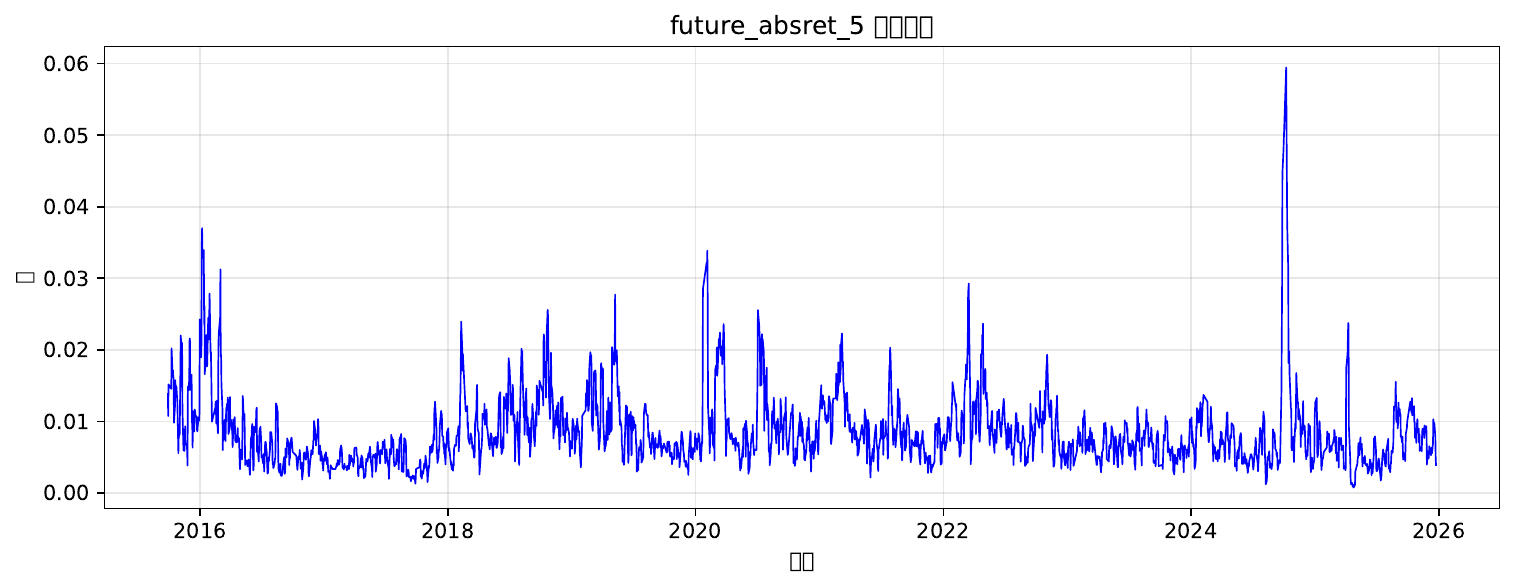
\includegraphics[width=0.85\textwidth]{figures/future_absret_5.png}
\caption{\texttt{future\_absret\_5}时间序列图}
\label{fig:future-absret}
\end{figure}

% 图2-2：future_logrv_20时间序列图
\begin{figure}[htbp]
\centering
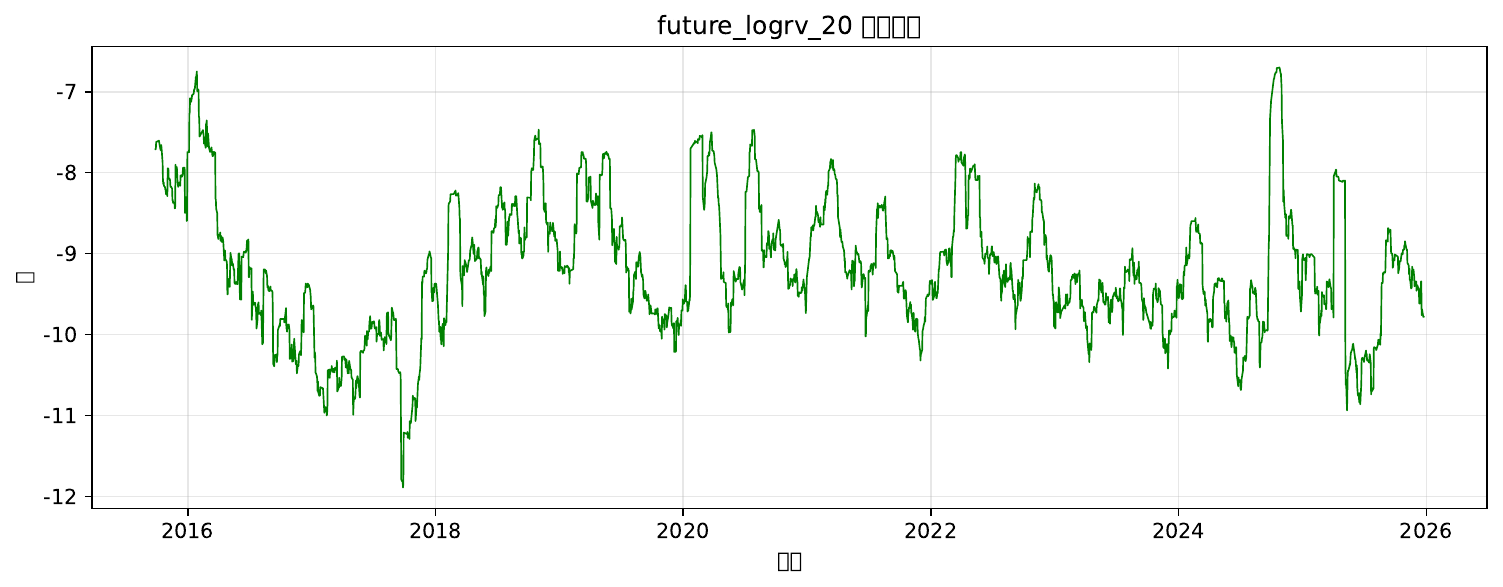
\includegraphics[width=0.85\textwidth]{figures/future_logrv_20.png}
\caption{\texttt{future\_logrv\_20}时间序列图}
\label{fig:future-logrv}
\end{figure}

% 图2-3：宏观变量时间序列图
\begin{figure}[htbp]
\centering
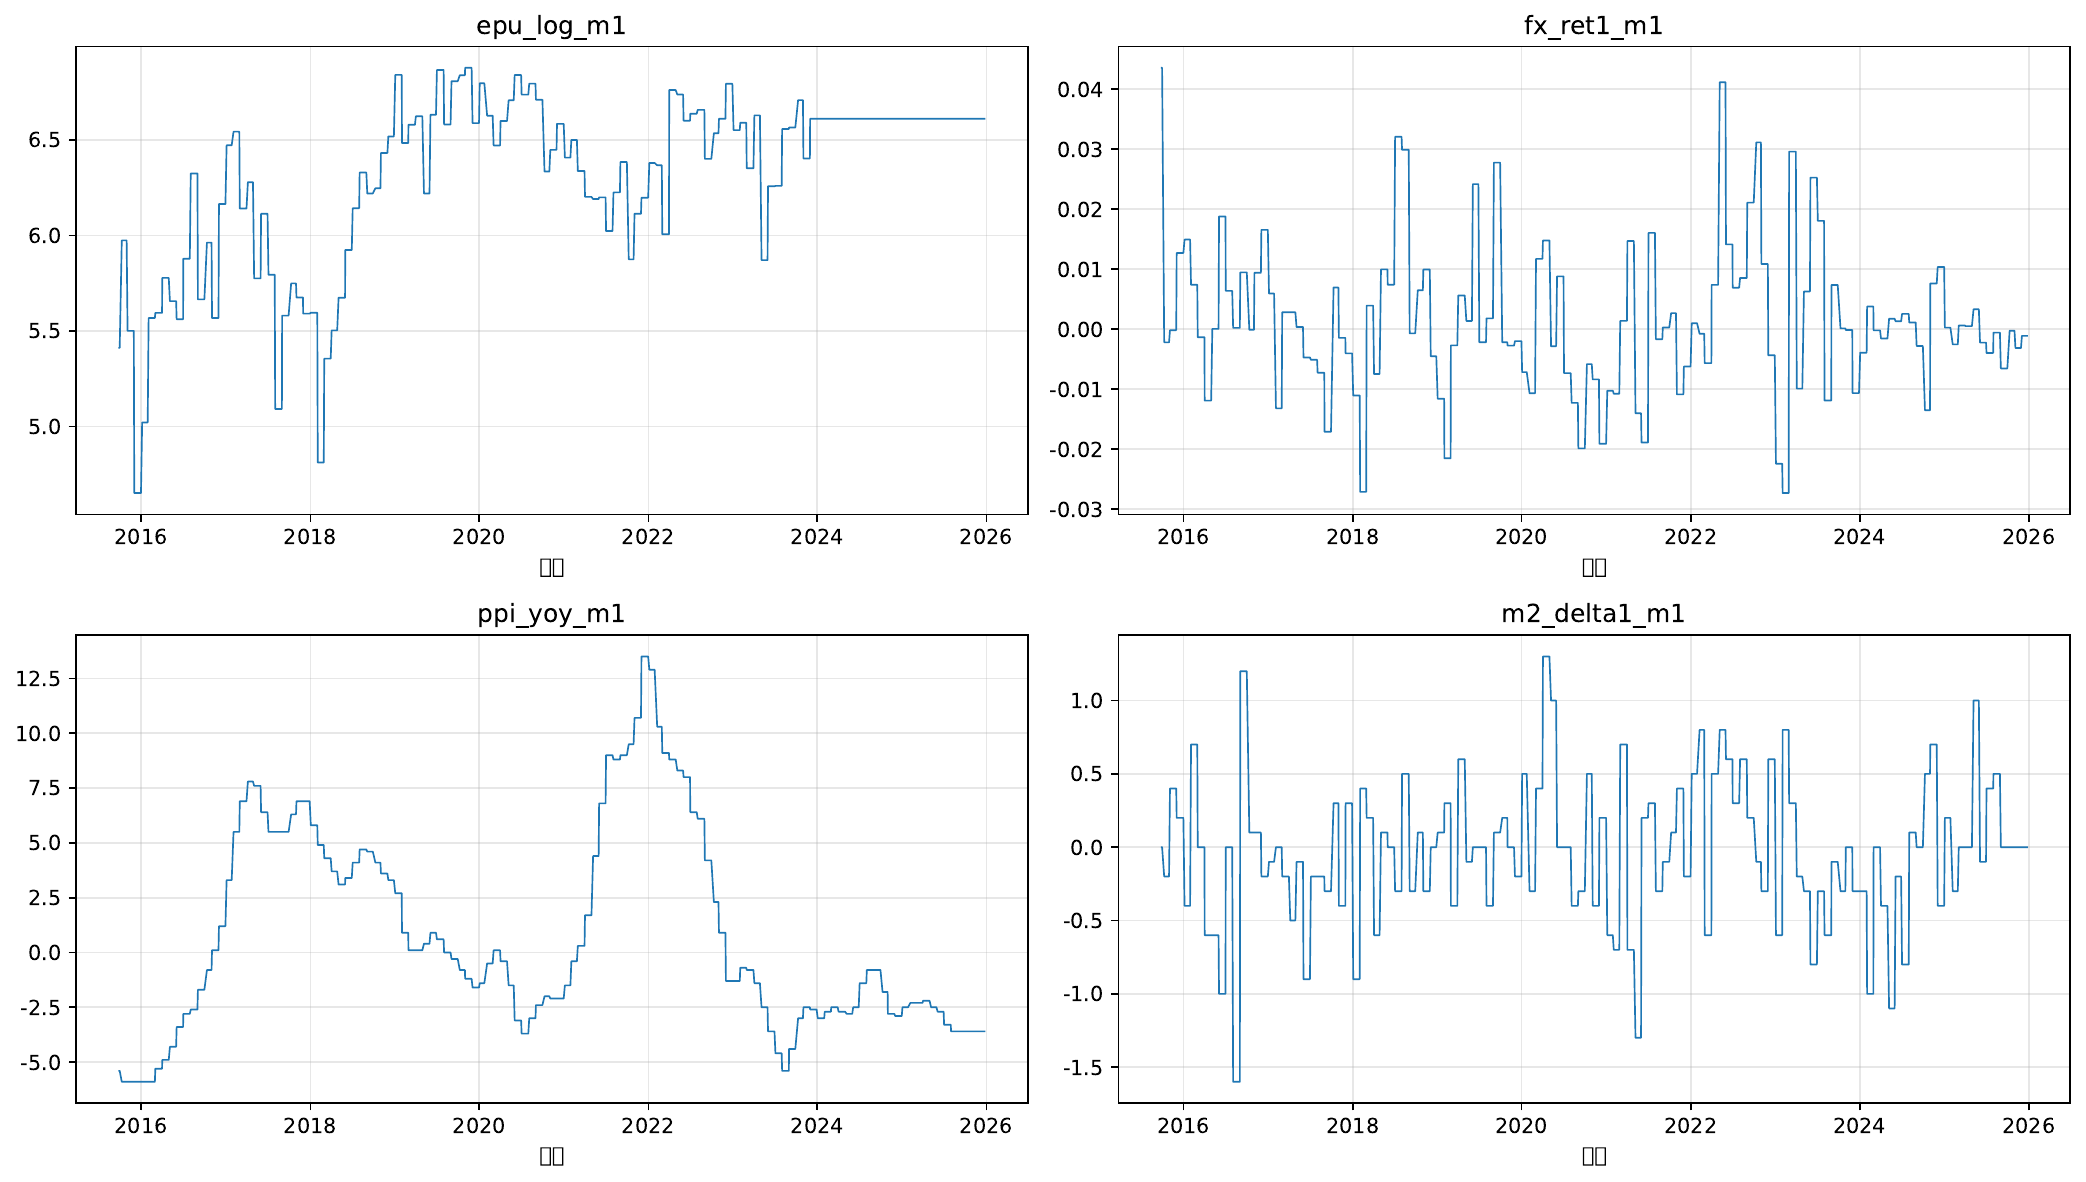
\includegraphics[width=0.85\textwidth]{figures/macro_variables.png}
\caption{宏观变量时间序列图}
\label{fig:macro-series}
\end{figure}

\subsection{相关性与初步关系检验}

相关性分析进一步说明，主因变量的主要信息首先来自历史状态变量本身。\texttt{future\_absret\_5}与\texttt{past\_absret\_5}的相关系数为0.897，与\texttt{past\_absret\_20}的相关系数为0.643，与\texttt{past\_absret\_60}的相关系数为0.444。这个结果非常直观地表明，未来一周平均波动幅度与过去5日和20日历史状态的联系最紧密，而60日尺度虽然仍有相关性，但强度已经明显下降。

与主因变量相比，宏观变量与\texttt{future\_absret\_5}的线性相关性整体较弱。\texttt{epu\_log\_m1}、\texttt{fx\_ret1\_m1}、\texttt{ppi\_yoy\_m1}与\texttt{future\_absret\_5}的相关系数绝对值都不高，这预示了宏观变量在正式回归中更可能表现为边际修正项，而不会成为主导性解释来源。辅助因变量\texttt{future\_logrv\_20}与其对应的\texttt{past\_logrv\_5}、\texttt{past\_logrv\_20}、\texttt{past\_logrv\_60}相关性极高，说明中期波动状态本身具有更强的持续性，这也解释了为何该因变量在样本外评估中表现得极好。

% 表2-3：future_absret_5与HAR状态变量相关系数矩阵
\begin{table*}[htbp]
\centering
\footnotesize
\caption{\texttt{future\_absret\_5}与HAR状态变量相关系数矩阵}
\label{tab:corr-absret}
\begin{tabular}{lcccc}
\topline
变量 & \texttt{future\_absret\_5} & \texttt{past\_absret\_5} & \texttt{past\_absret\_20} & \texttt{past\_absret\_60} \\
\midline
\texttt{future\_absret\_5} & 1.000 & 0.897 & 0.643 & 0.444 \\
\texttt{past\_absret\_5} & 0.897 & 1.000 & 0.693 & 0.468 \\
\texttt{past\_absret\_20} & 0.643 & 0.693 & 1.000 & 0.740 \\
\texttt{past\_absret\_60} & 0.444 & 0.468 & 0.740 & 1.000 \\
\bottomline
\end{tabular}
\end{table*}

% 表2-4：future_absret_5与宏观变量相关系数矩阵
\begin{table*}[htbp]
\centering
\footnotesize
\caption{\texttt{future\_absret\_5}与宏观变量相关系数矩阵}
\label{tab:corr-macro}
\begin{tabular}{lcccc}
\topline
变量 & \texttt{future\_absret\_5} & \texttt{epu\_log\_m1} & \texttt{fx\_ret1\_m1} & \texttt{ppi\_yoy\_m1} \\
\midline
\texttt{future\_absret\_5} & 1.000 & -0.074 & 0.060 & -0.065 \\
\texttt{epu\_log\_m1} & -0.074 & 1.000 & -0.041 & -0.145 \\
\texttt{fx\_ret1\_m1} & 0.060 & -0.041 & 1.000 & 0.034 \\
\texttt{ppi\_yoy\_m1} & -0.065 & -0.145 & 0.034 & 1.000 \\
\bottomline
\end{tabular}
\end{table*}

% 表2-5：future_logrv_20与HAR状态变量相关系数矩阵
\begin{table*}[htbp]
\centering
\footnotesize
\caption{\texttt{future\_logrv\_20}与HAR状态变量相关系数矩阵}
\label{tab:corr-logrv}
\begin{tabular}{lcccc}
\topline
变量 & \texttt{future\_logrv\_20} & \texttt{past\_logrv\_5} & \texttt{past\_logrv\_20} & \texttt{past\_logrv\_60} \\
\midline
\texttt{future\_logrv\_20} & 1.000 & 0.976 & 0.988 & 0.983 \\
\texttt{past\_logrv\_5} & 0.976 & 1.000 & 0.977 & 0.961 \\
\texttt{past\_logrv\_20} & 0.988 & 0.977 & 1.000 & 0.986 \\
\texttt{past\_logrv\_60} & 0.983 & 0.961 & 0.986 & 1.000 \\
\bottomline
\end{tabular}
\end{table*}

\subsection{样本特征总结与对后续模型的支撑}

从数据特征来看，本文的经验分析具备几个明显前提。主因变量存在较强右偏和厚尾，因此需要在回归阶段使用稳健标准误处理潜在异方差。主因变量与HAR历史状态变量之间具有较高相关性，为构建基准动态模型提供了充分依据。宏观变量与主因变量的线性相关性整体不强，说明后续的HARX扩展更适合作为增量检验，而不适合被预设为显著提高样本外表现的模型。辅助目标\texttt{future\_logrv\_20}与历史状态变量的高度相关，则提示其中期状态持续性极强，更适合作为稳健性对照而非主结论来源。

% 第三章 研究设计

\section{研究设计}

\subsection{研究设计概括}

本文围绕"宏观经济指标如何形成沪深300指数未来收益预期，以及实际收益偏离该预期的机制"展开实证分析，整体采用两阶段研究框架。第一阶段以宏观经济变量为核心信息集，构建沪深300指数未来5日与60日累计收益率的条件预期；第二阶段在此基础上，以实际累计收益率与条件预期收益率之差构造异常收益及其绝对值，并进一步检验市场状态变量对收益偏离的解释作用。

在第一阶段，MIDAS 混频回归用于处理月度宏观变量与日度金融收益率之间的频率不一致问题。考虑到宏观变量对未来收益的影响既存在时滞，又可能呈现不同的传导强度，模型通过参数化权重函数压缩过去若干期低频宏观信息，进而形成不同期限下的条件预期收益率\cite{ghysels2004midas,zheng2013midas}。进入精简多变量模型前，先在训练集上完成 VIF 检验，对共线性水平较高的变量进行剔除或替换，再结合样本外预测表现和经济含义确定保留变量集合。

由第一阶段模型生成的条件预测值构成未来5日和60日收益率的宏观预期水平。基于此，本文构造异常收益 $AR_t^{(h)}$ 以及异常收益绝对值 $AbsAR_t^{(h)}$，其中 $h=5,60$。主结果变量采用异常收益绝对值，以刻画市场相对于宏观预期的偏离强度；方向性异常收益则作为补充结果变量，用于观察偏离方向。

第二阶段采用分组嵌套回归识别异常收益偏离的形成机制。情绪与风险感知变量、资金与杠杆交易变量、流动性与交易状态变量依次进入回归方程。每新增一组变量，除比较调整后 $R^2$ 的变化之外，还对新增变量组进行联合显著性检验，以判断该组变量是否对模型解释力形成实质增量。完整嵌套模型估计完成后，再使用 LASSO 在标准化变量集合上进行辅助筛选，将系数压缩为零的变量排除在综合模型之外。最终综合模型采用具有清晰经济解释的变量集合，并继续使用 OLS 配合 HAC 稳健标准误报告结果。

% 图3-1：研究设计总体框架图
\begin{figure}[htbp]
\centering
\begin{tikzpicture}[
    node distance=0.8cm and 1.2cm,
    box1/.style={rectangle, rounded corners, draw=blue!60, fill=blue!5, thick, minimum width=3cm, minimum height=1cm, align=center, font=\small},
    box2/.style={rectangle, rounded corners, draw=green!60, fill=green!5, thick, minimum width=3cm, minimum height=1cm, align=center, font=\small},
    arrow/.style={-{Stealth[length=2mm]}, thick},
    label/.style={font=\small\bfseries}
]

% 阶段标签（左侧）
\node[label, blue!70] at (-2,0) {第一阶段};
\node[label, green!70] at (-2,-2.2) {第二阶段};

% 第一阶段
\node[box1] (macro) {宏观变量};
\node[box1, right=of macro] (midas) {MIDAS加权};
\node[box1, right=of midas] (exp) {条件预期收益};

% 第二阶段
\node[box2, below=1.5cm of macro] (market) {市场状态变量};
\node[box2, below=1.5cm of midas] (ar) {异常收益};
\node[box2, below=1.5cm of exp] (reg) {分组嵌套回归};

% 箭头
\draw[arrow, blue!60] (macro) -- (midas);
\draw[arrow, blue!60] (midas) -- (exp);
\draw[arrow, blue!60] (exp) -- (ar);
\draw[arrow, green!60] (market) -- (reg);
\draw[arrow, green!60] (ar) -- (reg);

\end{tikzpicture}
\caption{研究设计总体框架图}
\label{fig:design_overview}
\end{figure}

\subsection{变量定义与数据处理}

本文以沪深300指数为研究对象，核心被解释变量为未来一定持有期内的累计收益率。设交易日 $t$ 的收盘价为 $P_t$，则日对数收益率定义为
\begin{equation}
r_t=\ln\left(\frac{P_t}{P_{t-1}}\right)
\label{eq:daily_return}
\end{equation}
在此基础上，分别构造未来5日与未来60日累计收益率：
\begin{equation}
R_t^{(h)}=\sum_{s=1}^{h}r_{t+s}=\ln\left(\frac{P_{t+h}}{P_t}\right),\qquad h\in\{5,60\}
\label{eq:cumulative_return}
\end{equation}
其中，$R_t^{(5)}$ 刻画短线收益表现，$R_t^{(60)}$ 对应相对更长的收益窗口。两个变量同时纳入分析，能够比较宏观信息在不同期限上的解释能力，也便于观察短线波动与长线趋势在形成机制上的差异。

第一阶段模型使用的宏观变量主要包括居民消费价格指数同比增速、工业生产者出厂价格指数同比增速、M2同比增速、经济政策不确定性指数以及美元兑人民币汇率。它们分别对应通胀环境、工业价格水平、货币条件、政策预期与外部金融约束等不同层面的宏观信息，能够较为全面地刻画市场所面对的基本面状态。考虑到这些变量大多以月度频率发布，而股票收益率以日频观测，月度数据采用"上一个完整月可得信息"与当前交易日对齐。若以 $m(t)$ 表示交易日 $t$ 所属月份，则任一月度变量 $X_j$ 在交易日 $t$ 的可用值写作
\begin{equation}
X_{j,t}^{M}=X_{j,m(t)-1}
\label{eq:macro_alignment}
\end{equation}
若在扩展检验中纳入 GDP，设 $q(t)$ 表示交易日 $t$ 所属季度，则其可用值表示为
\begin{equation}
GDP_t^{Q}=GDP_{q(t)-1}
\label{eq:gdp_alignment}
\end{equation}

第二阶段的解释变量不再承担生成收益预期的功能，而用于说明实际收益为何偏离宏观预期。围绕这一目的，本文将相关变量划分为三类。第一类是情绪与风险感知变量，包括情绪标准分与隐含波动率指数，它们更接近市场参与者的主观预期与风险定价状态。第二类是资金与杠杆交易变量，包括北向资金净流入和融资融券余额，反映不同类型交易资金对价格的推动作用。第三类为流动性与交易状态变量，包括 Amihud 非流动性指标、20日动量和日内振幅，用于刻画市场微观结构状态以及短期交易拥挤程度。第二阶段所有解释变量统一采用滞后一期形式进入回归，以减弱同期反馈关系带来的干扰。

预处理流程与样本划分同步进行。训练集内完成缩尾阈值估计、标准化参数计算以及后续的变量筛选和模型训练，测试集使用训练集参数完成映射。第二阶段连续解释变量的标准化处理形式为
\begin{equation}
Z(x_t)=\frac{x_t-\bar{x}_{train}}{s_{train}}
\label{eq:standardization_train}
\end{equation}
其中，$\bar{x}_{train}$ 和 $s_{train}$ 分别表示训练集均值和训练集标准差。标准化之后，各变量系数可以在统一尺度下进行比较，便于识别哪一类因素对异常收益偏离的影响更为突出。

\subsection{第一阶段：基于 MIDAS 的预期收益模型}

本文第一阶段的目标，是利用宏观变量构造未来5日与60日累计收益率的条件预期。由于月度宏观指标与日度收益率之间存在明显的频率不一致问题，若直接将低频变量以普通滞后项形式放入日频回归，既无法充分体现宏观信息的持续作用，也难以刻画不同滞后期信息的相对重要性。基于此，本文采用 MIDAS 混频回归框架，将过去若干期低频宏观变量通过参数化权重函数压缩为日频时点上的有效解释量，再用于未来收益率预测\cite{ghysels2004midas,ghysels2007midas}。

% 图3-2：MIDAS建模结构
\begin{figure}[htbp]
\centering
\begin{tikzpicture}[
    node distance=0.8cm and 1.5cm,
    box/.style={rectangle, rounded corners, draw=blue!60, fill=blue!5, thick, minimum width=2cm, minimum height=0.7cm, align=center, font=\small},
    sum/.style={circle, draw=blue!60, fill=blue!10, thick, minimum size=0.7cm, font=\small},
    arrow/.style={-{Stealth[length=2mm]}, thick, blue!60}
]

% Beta权重函数标注（顶部）
\node[font=\small] at (3.5,4) {Beta权重函数};

% 月度变量节点
\node[box] (cpi) {CPI$_{t-1}$};
\node[box, below=of cpi] (ppi) {PPI$_{t-1}$};
\node[box, below=of ppi] (m2) {M2$_{t-1}$};
\node[box, below=of m2] (epu) {EPU$_{t-1}$};
\node[box, below=of epu] (usd) {USD$_{t-1}$};

% 权重节点
\node[sum, right=of cpi] (w1) {$w_1$};
\node[sum, right=of ppi] (w2) {$w_2$};
\node[sum, right=of m2] (w3) {$w_3$};
\node[sum, right=of epu] (w4) {$w_4$};
\node[sum, right=of usd] (w5) {$w_5$};

% MIDAS加权
\node[box, right=of w3] (midas) {MIDAS加权项};

% 预测
\node[box, right=of midas] (pred) {$\widehat{R}_t^{(h)}$};

% 箭头
\foreach \i in {1,...,5} {
    \draw[arrow] (w\i) -- (midas);
}
\draw[arrow] (cpi) -- (w1);
\draw[arrow] (ppi) -- (w2);
\draw[arrow] (m2) -- (w3);
\draw[arrow] (epu) -- (w4);
\draw[arrow] (usd) -- (w5);
\draw[arrow] (midas) -- (pred);

\end{tikzpicture}
\caption{MIDAS建模结构示意图}
\label{fig:midas_structure}
\end{figure}

对于任一月度宏观变量 $X_j$，其在预测窗口 $h$ 下的 MIDAS 加权项定义为
\begin{equation}
\mathcal{M}_{j,t}^{(h)}=\sum_{\ell=0}^{K_j-1}w_{j,\ell}^{(h)}(\theta_{j,h})X_{j,m(t)-1-\ell}
\label{eq:midas_weighted}
\end{equation}
其中，$K_j$ 表示变量 $X_j$ 纳入的月度滞后长度，本文统一取 $K_j=12$；$w_{j,\ell}^{(h)}(\theta_{j,h})$ 为对应的权重函数，用以刻画不同月份宏观信息对未来收益率的影响强度。主模型使用 Beta 权重函数：
\begin{equation}
w_{j,\ell}(a_{j,h},b_{j,h})=\frac{\left(\frac{\ell+1}{K_j+1}\right)^{a_{j,h}-1}\left(1-\frac{\ell+1}{K_j+1}\right)^{b_{j,h}-1}}{\sum_{r=0}^{K_j-1}\left(\frac{r+1}{K_j+1}\right)^{a_{j,h}-1}\left(1-\frac{r+1}{K_j+1}\right)^{b_{j,h}-1}}
\label{eq:beta_weights}
\end{equation}
并满足
\begin{equation}
\sum_{\ell=0}^{K_j-1}w_{j,\ell}(a_{j,h},b_{j,h})=1
\label{eq:weight_sum}
\end{equation}

在具体估计时，本文首先分别构建单变量 MIDAS 模型。对于宏观变量 $X_j$，未来 $h$ 日累计收益率的单变量预测方程写作
\begin{equation}
R_t^{(h)}=\alpha_{j,h}+\beta_{j,h}\mathcal{M}_{j,t}^{(h)}+u_{j,t}^{(h)},\qquad h\in\{5,60\}
\label{eq:single_midas}
\end{equation}
这一阶段逐一考察不同宏观变量在短线与长线收益预测中的独立作用。单变量模型结果除报告系数估计值、t统计量和显著性水平外，还将展示预测值与真实值的可视化对比，以及对应的残差图和残差时间序列图，用于识别拟合偏差和时段性误差聚集。

完成单变量估计后，本文在训练集上对候选宏观变量计算 VIF，并结合样本内统计表现、样本外预测效果和变量的经济含义构建精简多变量 MIDAS 模型。表~\ref{tab:stage1_results}报告了第一阶段主要模型的估计结果。

% 表3-1：第一阶段MIDAS模型估计结果
\begin{table}[htbp]
\centering
\caption{第一阶段 MIDAS 模型估计结果}
\label{tab:stage1_results}
\small
\begin{tabular}{lcccc}
\topline
\textbf{模型} & \textbf{预测窗口} & \textbf{$R^2$(样本内)} & \textbf{$R^2$(样本外)} & \textbf{RMSE} \\
\midline
单变量最优 & 5日 & 0.0063 & 0.0003 & 0.0265 \\
精简多变量 & 5日 & 0.0076 & -0.0041 & 0.0266 \\
\midline
单变量最优 & 60日 & 0.0528 & 0.0329 & 0.0799 \\
精简多变量 & 60日 & 0.1110 & -0.1148 & 0.0859 \\
\bottomline
\end{tabular}
\end{table}

注：单变量最优模型基于经济政策不确定性指数（EPU）构建。精简多变量模型经VIF筛选后仅保留PPI。
\begin{equation}
R_t^{(h)}=\alpha_h+\sum_{j=1}^{J^*}\beta_{j,h}\mathcal{M}_{j,t}^{(h)}+u_t^{(h)}
\label{eq:multi_midas}
\end{equation}
其中 $J^*\leq 4$。由该模型得到的拟合值即构成未来 $h$ 日累计收益率的宏观预期：
\begin{equation}
\widehat{R}_t^{(h)}=\hat{\alpha}_h+\sum_{j=1}^{J^*}\hat{\beta}_{j,h}\mathcal{M}_{j,t}^{(h)}
\label{eq:expected_return}
\end{equation}

第一阶段 MIDAS 模型采用非线性最小二乘法进行参数估计。对于任意预测窗口 $h$，其目标函数为
\begin{equation}
SSR_h(\Theta_h)=\sum_t\left(R_t^{(h)}-\widehat{R}_t^{(h)}\right)^2
\label{eq:ssr}
\end{equation}
其中 $\Theta_h$ 包含截距、回归系数及权重函数参数。针对未来5日和未来60日收益率，本文分别独立估计模型，而不通过一步预测模型递推生成多步预测值。除数值指标外，实证展示中还将对代表性的单变量模型与精简多变量模型绘制"真实值—预测值"折线图，以直接比较两种模型在不同收益窗口中的拟合与预测表现。

% 表3-1：第一阶段变量与窗口设定
\begin{table}[htbp]
\centering
\caption{第一阶段变量与窗口设定}
\label{tab:stage1_settings}
\begin{tabular}{p{3cm}p{2.5cm}p{2cm}p{3cm}p{2cm}}
\topline
\textbf{变量} & \textbf{频率} & \textbf{滞后长度} & \textbf{预测窗口} & \textbf{估计方法} \\
\midline
CPI同比增速 & 月度 & $K=12$ & $h=5,60$日 & NLS \\
PPI同比增速 & 月度 & $K=12$ & $h=5,60$日 & NLS \\
M2同比增速 & 月度 & $K=12$ & $h=5,60$日 & NLS \\
EPU指数 & 月度 & $K=12$ & $h=5,60$日 & NLS \\
美元兑人民币汇率 & 月度 & $K=12$ & $h=5,60$日 & NLS \\
\bottomline
\end{tabular}
\end{table}

在扩展检验中，本文进一步将季度 GDP 增速纳入第一阶段模型，以考察实体经济总量指标能否在月度变量之外提供额外信息。GDP 的 MIDAS 加权项定义为
\begin{equation}
\mathcal{Q}_{GDP,t}^{(h)}=\sum_{\ell=0}^{K_g-1}v_{\ell}^{(h)}(\psi_h)GDP_{q(t)-1-\ell}
\label{eq:gdp_midas}
\end{equation}
并设 $K_g=4$。扩展模型可写为
\begin{equation}
R_t^{(h)}=\alpha_h+\sum_{j=1}^{J^*}\beta_{j,h}\mathcal{M}_{j,t}^{(h)}+\gamma_h\mathcal{Q}_{GDP,t}^{(h)}+u_t^{(h)}
\label{eq:extended_midas}
\end{equation}
这一设定用于检验主模型结果在引入季度总量信息后是否依然稳健。

% 新增图：真实值与预测值对比图（5日窗口）
\begin{figure}[htbp]
\centering

\includegraphics[width=0.9\textwidth]{figures/true_pred_5d.png}
\caption{未来5日累计收益率的真实值与预测值对比}
\label{fig:true_pred_5d}
\end{figure}

% 新增图：真实值与预测值对比图（60日窗口）
\begin{figure}[htbp]
\centering

\includegraphics[width=0.9\textwidth]{figures/true_pred_60d.png}
\caption{未来60日累计收益率的真实值与预测值对比}
\label{fig:true_pred_60d}
\end{figure}

% 新增图：第一阶段残差诊断图
\begin{figure}[htbp]
\centering

\includegraphics[width=0.9\textwidth]{figures/residual_stage1.png}
\caption{第一阶段 MIDAS 模型残差诊断图}
\label{fig:residual_stage1}
\end{figure}

\subsection{第二阶段：异常收益偏离的分组嵌套回归}

第一阶段得到的是给定宏观信息集下未来收益率的条件预期，实际市场收益并不必然完全围绕这一基准运行。尤其在情绪波动、资金快速流动或流动性收缩的情况下，市场表现往往会偏离宏观变量所隐含的收益水平。基于这一考虑，本文在第二阶段转向考察实际收益偏离宏观预期的形成机制。

首先，根据第一阶段的预测值构造异常收益：
\begin{equation}
AR_t^{(h)}=R_t^{(h)}-\widehat{R}_t^{(h)},\qquad h\in\{5,60\}
\label{eq:ar_def}
\end{equation}
当 $AR_t^{(h)}>0$ 时，说明实际累计收益高于宏观预期；反之则表明实际收益低于宏观预期。本文进一步定义异常收益绝对值，用以刻画偏离强度：
\begin{equation}
AbsAR_t^{(h)}=\left|AR_t^{(h)}\right|
\label{eq:absar_def}
\end{equation}
异常收益绝对值更适合刻画市场异动程度，也更贴近第二阶段关于偏离放大机制的研究目标。因此，主结果部分以 $AbsAR_t^{(5)}$ 和 $AbsAR_t^{(60)}$ 为因变量，补充分析中再讨论 $AR_t^{(5)}$ 和 $AR_t^{(60)}$ 的方向性结果。

在模型设定上，第二阶段采用分组嵌套回归。第一组变量为情绪与风险感知变量，包括情绪标准分和隐含波动率指数。相应回归式写为
\begin{equation}
Y_t^{(h)}=\alpha_{0,h}+\alpha_{1,h}sentiment\_zscore_{t-1}+\alpha_{2,h}ivix_{t-1}+\varepsilon_t^{(h,1)}
\label{eq:model1}
\end{equation}
其中 $Y_t^{(h)}$ 表示第二阶段因变量，在主结果中取 $AbsAR_t^{(h)}$，在补充结果中取 $AR_t^{(h)}$。

第二步加入资金与杠杆交易变量，即北向资金净流入和融资融券余额，得到第二个嵌套模型：
\begin{equation}
\begin{aligned}
Y_t^{(h)}=\beta_{0,h}&+\beta_{1,h}sentiment\_zscore_{t-1}+\beta_{2,h}ivix_{t-1}\\
&+\beta_{3,h}north\_flow_{t-1}+\beta_{4,h}margin\_balance_{t-1}+\varepsilon_t^{(h,2)}
\end{aligned}
\label{eq:model2}
\end{equation}

第三步再纳入流动性与交易状态变量，包括 Amihud 非流动性指标、20日动量和日内振幅，形成完整的嵌套模型：
\begin{equation}
\begin{aligned}
Y_t^{(h)}=\gamma_{0,h}&+\gamma_{1,h}sentiment\_zscore_{t-1}+\gamma_{2,h}ivix_{t-1}\\
&+\gamma_{3,h}north\_flow_{t-1}+\gamma_{4,h}margin\_balance_{t-1}\\
&+\gamma_{5,h}amihud_{t-1}+\gamma_{6,h}momentum_{20d,t-1}\\
&+\gamma_{7,h}intraday\_range_{t-1}+\varepsilon_t^{(h,3)}
\end{aligned}
\label{eq:model3}
\end{equation}

在模型I至模型III之间，本文对新增变量组进行联合显著性检验，并结合调整后 $R^2$ 的变化衡量各组变量的边际贡献。若新增变量组在统计上显著，且模型拟合有明显改善，则说明该组变量对异常收益偏离具有独立解释力。这样得到的增量检验结果，可以补充单纯依赖 $R^2$ 变化所带来的判断局限。

% 图3-6：第二阶段分组嵌套回归结构
\begin{figure}[htbp]
\centering
\begin{tikzpicture}[
    node distance=0.3cm and 0.8cm,
    box/.style={rectangle, rounded corners, draw=green!60, fill=green!5, thick, minimum width=3cm, minimum height=0.6cm, align=center, font=\small},
    arrow/.style={-{Stealth[length=2mm]}, thick, green!60}
]

% 模型1
\node[box] (m1) {模型I：情绪与风险感知\\情绪标准分 + iVIX};

% 模型2
\node[box, below=0.4cm of m1] (m2) {模型II：加入资金与杠杆\\+ 北向资金 + 融资融券};

% 模型3
\node[box, below=0.4cm of m2] (m3) {模型III：完整模型\\+ Amihud + 动量 + 振幅};

% 模型4
\node[box, below=0.4cm of m3] (m4) {综合模型：LASSO筛选\\保留非零系数变量};

% 箭头
\draw[arrow] (m1) -- (m2);
\draw[arrow] (m2) -- (m3);
\draw[arrow] (m3) -- (m4);

% 因变量
\node[left=1.5cm of m2, align=center, font=\small] (y) {因变量：\\$AbsAR_t^{(5)}$\\$AbsAR_t^{(60)}$};
\draw[arrow, blue!60] (y) -- (m1);
\draw[arrow, blue!60] (y) -- (m2);
\draw[arrow, blue!60] (y) -- (m3);

% 标准误标注
\node[right=1.5cm of m2, align=center, font=\small] (se) {Newey--West\\HAC标准误};
\draw[arrow, gray] (m1) -- (se);
\draw[arrow, gray] (m2) -- (se);
\draw[arrow, gray] (m3) -- (se);
\draw[arrow, gray] (m4) -- (se);

\end{tikzpicture}
\caption{第二阶段分组嵌套回归结构图}
\label{fig:nested_regression}
\end{figure}

完整嵌套模型估计完成后，本文再对所有标准化市场状态变量应用 LASSO 回归，通过交叉验证选择惩罚参数 $\lambda$，以识别系数收缩为零的变量。表~\ref{tab:stage2_results}报告了第二阶段分组嵌套回归的估计结果。

% 表3-2：第二阶段分组嵌套回归估计结果
\begin{table}[htbp]
\centering
\caption{第二阶段分组嵌套回归估计结果}
\label{tab:stage2_results}
\small
\begin{tabular}{lcccc}
\topline
\textbf{预测窗口} & \textbf{模型} & \textbf{调整后$R^2$} & \textbf{增量解释力} & \textbf{LASSO保留变量} \\
\midline
5日 & 模型I（情绪） & 0.0604 & -- & -- \\
5日 & 模型II（+资金） & 0.0614 & 0.0010 & -- \\
5日 & 模型III（+流动性） & 0.0630 & 0.0016 & -- \\
5日 & 综合模型 & 0.0643 & -- & ivix, north\_flow, margin, turnover \\
\midline
60日 & 模型I（情绪） & 0.0014 & -- & -- \\
60日 & 模型II（+资金） & 0.0108 & 0.0094 & -- \\
60日 & 模型III（+流动性） & 0.0140 & 0.0032 & -- \\
60日 & 综合模型 & 0.0014 & -- & ivix \\
\bottomline
\end{tabular}
\end{table}

注：增量解释力为相对于前一模型的调整后$R^2$变化。LASSO筛选基于交叉验证选择惩罚参数。
\begin{equation}
Y_t^{(h)}=\delta_{0,h}+\sum_{k=1}^{K_h^*}\delta_{k,h}W_{k,t-1}+\varepsilon_t^{(h,4)}
\label{eq:model4}
\end{equation}
其中 $W_{k,t-1}$ 为在完整嵌套模型与 LASSO 筛选程序中同时得到支持的变量集合，$K_h^*$ 为保留变量个数。

第二阶段结果展示包括各模型的系数估计值、t统计量、显著性水平、调整后 $R^2$、新增变量组联合检验结果，以及残差拟合图和残差时间序列图。这样既可以展示变量方向和边际效应，也可以检验模型误差是否存在明显的时段性偏离。

由于未来5日和未来60日累计收益率都采用了重叠窗口构造方式，由此形成的异常收益及其绝对值序列通常存在明显的序列相关。为保证推断结果稳健，第二阶段所有回归均采用OLS估计，并使用 Newey--West HAC 稳健标准误对统计量进行修正。对于5日窗口，HAC 滞后阶数取4；对于60日窗口，滞后阶数取59。

% 新增图：第二阶段残差诊断图
\begin{figure}[htbp]
\centering

\includegraphics[width=0.9\textwidth]{figures/residual_stage2.png}
\caption{第二阶段分组嵌套回归残差诊断图}
\label{fig:residual_stage2}
\end{figure}

% 新增图：LASSO交叉验证误差图
\begin{figure}[htbp]
\centering

\includegraphics[width=0.9\textwidth]{figures/lasso_cv.png}
\caption{LASSO 惩罚参数选择结果}
\label{fig:lasso_cv}
\end{figure}

% 新增图：LASSO系数路径图
\begin{figure}[htbp]
\centering

\includegraphics[width=0.9\textwidth]{figures/lasso_path.png}
\caption{第二阶段变量的 LASSO 系数路径图}
\label{fig:lasso_path}
\end{figure}

% 新增图：分组嵌套回归边际解释力图
\begin{figure}[htbp]
\centering

\includegraphics[width=0.9\textwidth]{figures/marginal_r2.png}
\caption{分组嵌套回归的边际解释力变化}
\label{fig:marginal_r2}
\end{figure}

\subsection{样本内与样本外评估}

第一阶段 MIDAS 模型的估计结果，需要同时从样本内拟合能力和样本外预测能力两个层面进行检验。仅凭样本内显著性并不足以说明宏观变量对未来收益率具有稳定预测作用，尤其在金融市场收益预测问题中，模型往往会在样本内表现良好，却在样本外递推中迅速减弱。因此，本文将样本内与样本外评估作为第一阶段实证分析中并行展开的两个部分\cite{campbell2008predicting,welch2008comprehensive}。

在样本内部分，本文首先报告单变量 MIDAS 模型与精简多变量 MIDAS 模型的参数估计结果，包括各变量的系数估计值、t统计量、显著性水平，以及模型的 $R^2$、调整后 $R^2$、AIC 和 BIC。宏观变量在5日与60日收益窗口下的拟合能力将通过表格和图形两种方式同时展示。表格部分用于比较统计指标，图形部分则绘制真实值与两类模型预测值的折线图，展示代表性区间内单变量最优模型、精简多变量模型与真实收益率之间的动态差异。

在样本外部分，本文采用扩展窗口法进行动态递推预测。将样本前60\%的区间设定为初始估计窗口，用于第一次参数估计；随后每向前推进一个预测时点，便将新观测纳入样本，重新估计模型，并生成该时点对应的未来5日或未来60日收益预测值。如此递推，直到覆盖全部样本外区间。设样本外区间记为 $OOS$，则在预测窗口 $h$ 下，样本外均方根误差定义为
\begin{equation}
RMSE_h=\sqrt{\frac{1}{T_{OOS}}\sum_{t\in OOS}\left(R_t^{(h)}-\hat{R}_t^{(h)}\right)^2}
\label{eq:rmse}
\end{equation}
平均绝对误差定义为
\begin{equation}
MAE_h=\frac{1}{T_{OOS}}\sum_{t\in OOS}\left|R_t^{(h)}-\hat{R}_t^{(h)}\right|
\label{eq:mae}
\end{equation}
进一步地，样本外 $R^2$ 定义为
\begin{equation}
R_{OS,h}^{2}=1-\frac{\sum_{t\in OOS}(R_t^{(h)}-\hat{R}_t^{(h)})^2}{\sum_{t\in OOS}(R_t^{(h)}-\bar{R}_h)^2}
\label{eq:r2os}
\end{equation}
其中 $\bar{R}_h$ 表示以样本内历史均值构造的基准预测值。

第二阶段的核心任务在于识别异常收益偏离的形成机制，因此其评估重点放在嵌套模型中各组变量加入后的边际解释力变化。对 $AbsAR_t^{(5)}$、$AbsAR_t^{(60)}$、$AR_t^{(5)}$ 和 $AR_t^{(60)}$，分别报告模型I、模型II、模型III和综合模型的系数估计值、HAC修正后的 t统计量、调整后 $R^2$、新增变量组联合检验统计量，以及残差诊断图。这样既能反映各类变量的独立作用，也能展示完整模型向综合模型收束的过程。

% 表3-2：评价指标说明
\begin{table}[htbp]
\centering
\caption{评价指标说明}
\label{tab:metrics}
\begin{tabular}{p{2.5cm}p{8cm}c}
\topline
\textbf{指标} & \textbf{计算公式} & \textbf{判断标准} \\
\midline
$R^2$/调整$R^2$ & $1-\frac{SSR}{SST}$，考虑自由度修正 & 越大越好 \\
AIC & $-2\ln(L)+2k$，$k$为参数个数 & 越小越好 \\
BIC & $-2\ln(L)+k\ln(n)$，含样本量惩罚 & 越小越好 \\
RMSE & $\sqrt{\frac{1}{T}\sum(y_t-\hat{y}_t)^2}$ & 越小越好 \\
MAE & $\frac{1}{T}\sum|y_t-\hat{y}_t|$ & 越小越好 \\
$R^2_{OS}$ & $1-\frac{\sum_{OOS}(y_t-\hat{y}_t)^2}{\sum_{OOS}(y_t-\bar{y})^2}$ & $>0$优于历史均值 \\
\bottomline
\end{tabular}
\end{table}

\subsection{稳健性检验}

为确保实证结论不依赖于某一特定设定，本文从模型形式、滞后结构、变量选择、样本构造和样本区间等多个方面展开稳健性检验。

第一类稳健性检验针对第一阶段 MIDAS 模型中的权重函数设定。主模型采用 Beta 权重函数，以刻画过去12个月宏观信息对未来收益率的动态影响。为检验结果是否过于依赖这一特定函数形式，进一步使用 Exponential Almon 权重函数重新估计单变量和精简多变量 MIDAS 模型。若主要宏观变量的符号、显著性以及样本外预测排序未发生实质变化，则说明结果对权重函数设定具有较好的稳健性。

第二类稳健性检验针对滞后长度设定。主模型统一采用12个月月度滞后窗口。为检验这一设定对结果的影响，进一步将月度变量的滞后长度分别调整为6个月和18个月，并重新估计对应模型。若主要变量在不同滞后长度下依然表现出相近的方向和预测能力，则说明主结果不依赖单一窗口长度。

第三类稳健性检验围绕宏观变量筛选程序展开。主模型中，精简多变量 MIDAS 的解释变量来自单变量表现、VIF 检验和样本外预测结果的联合筛选。稳健性检验中，分别采用更严格的 VIF 阈值、不同的变量保留数量上限，以及加入 GDP 季度加权项的扩展设定进行比较，以检验变量选择规则是否影响主要结论。

第四类稳健性检验围绕收益窗口构造方式展开。由于未来5日和未来60日累计收益率采用重叠窗口构造，相邻观测之间共享部分收益信息。为此，在主结果采用 HAC 标准误修正之外，进一步构造非重叠收益窗口，分别形成5日和60日非重叠收益序列，并在相应样本上重新估计第一阶段和第二阶段模型。若主要结论在非重叠样本下仍保持方向一致，则说明结果不依赖重叠窗口带来的统计特征。

第五类稳健性检验关注样本期间的异质性。考虑到2015年以来中国资本市场经历了多次环境变化，不同时期的宏观变量传导方式、资金结构和交易风格都可能存在差异，本文按年份或相邻年份组合划分子样本，对主要模型分别进行重新估计，并比较不同子区间中的参数方向、显著性及预测能力。

第六类稳健性检验针对第二阶段综合模型的筛选程序。主文中综合模型依据完整嵌套模型中的变量显著性、调整后 $R^2$ 提升幅度以及 LASSO 非零系数结果共同确定。稳健性部分进一步比较不同惩罚参数选择规则、不同显著性门槛以及是否保留边界变量的结果差异，考察最终保留下来的核心变量是否稳定。


% 参考文献
\newpage
\bibliography{references}

\end{document}
